\documentclass{beamer}

%\usepackage{default}
%\usetheme{Berkeley}
\usetheme{Ilmenau}
\usecolortheme{beaver}
\usepackage[utf8]{inputenc}
\usepackage{caption}
\usepackage{pslatex}
\usepackage{textpos}
\usepackage{tikz}
%\useoutertheme{split}
%\useoutertheme{sidebar}
\usepackage{graphicx}
\pgfdeclareimage[height=2.35ex, width=2.2\baselineskip]{barcmini}{../PICS/barc_logo_circle.png}
\logo{\pgfuseimage{barcmini}}
\setbeamertemplate{sidebar right}{} %
\setbeamertemplate{footline}{\raisebox{-1ex}{\pgfuseimage{barcmini}}
    \usebeamerfont{date in head/foot} \@CERN \;\;\;\; \insertshortdate{}\hfill 
    \usebeamerfont{author in head/foot}\insertshortauthor{}\hfill
    \usebeamertemplate{navigation symbols}\hfill 
    \insertframenumber{}/\inserttotalframenumber
}
%\setbeamertemplate{navigation symbols}{}
\title{TARC Analysis using Geant4 and ADS at BARC}
\author{Abhijit Bhattacharyya}
\institute{Bhabha Atomic Research Center \\ Mumbai INDIA}
\date{\today}
%\logo{
\includegraphics[height=1cm,width=1cm]{../PICS/barc_logo_circle.png}}
\begin{document}
    \begin{frame}
        \maketitle
    \end{frame}
    
    \begin{frame}
        \frametitle{Outline}
        \tableofcontents [part=1, pausesections]
    \end{frame}

    \begin{frame}
      \frametitle{Idea for Indian ADS}
      \begin{figure}
        \includegraphics[height=65mm, width=100m]{../PICS/ADSPlan.ppm}
        \label{fig:ADSPlan}
        \caption{Basic scheme to burn Thorium with ADS.}
      \end{figure}
    \end{frame}

    
    \begin{frame}
      \frametitle{Fuel fraction}
      \begin{figure}
        \includegraphics[height=65mm, width=100m]{../PICS/ThUConsumption.ppm}
        \label{fig:ADSPlan}
        \caption{Consumption of fuel.}
      \end{figure}
    \end{frame}
    
    
    \begin{frame}
      \frametitle{50keV Ion Source :: ADS BARC INDIA}
      \begin{figure}
        \includegraphics[height=65mm, width=100m]{../PICS/50keV\_Ion\_Source.png}
        \label{fig:50keVionSource}
        \caption{50 keV Ion source}
      \end{figure}
    \end{frame}

    \begin{frame}
      \frametitle{ADS Target Testing Facility :: ADS BARC INDIA}
      \begin{figure}
        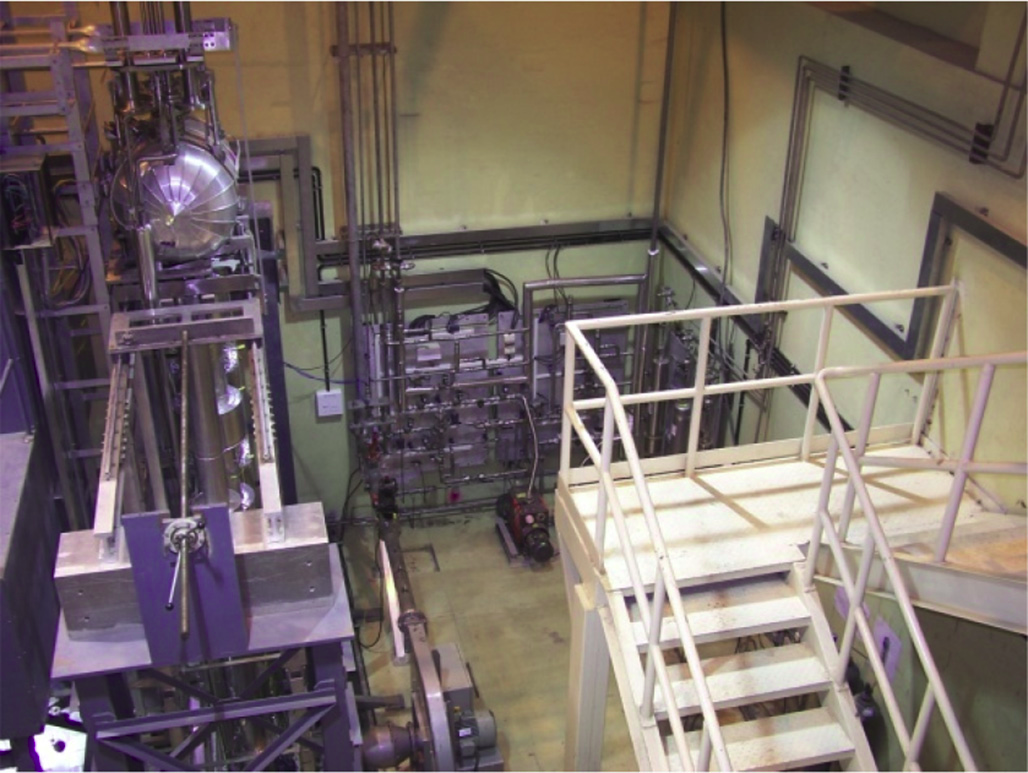
\includegraphics[height=65mm, width=100m]{../PICS/ADS_Target_Testing_Facility.png}
        \label{fig:ADSTARGET}
        \caption{ADS Target testing Facility}
      \end{figure}
    \end{frame}

    \begin{frame}
      \frametitle{RFQ Assembly with RF coupler and bending magnets :: ADS BARC INDIA}
      \begin{figure}
        \includegraphics[height=65mm, width=100m]{../PICS/RFQ\_Assembly\_with\ RFcoupler\_bending\_magnet.png}
        \label{fig:RFQAssem}
        \caption{RFQ Assembly with RF coupler and bending magnets}
      \end{figure}
    \end{frame}
    
    \begin{frame}
        \frametitle{Distribution of Neutron Energy Deposition}
        \begin{figure}
            \begin{tabular}{cc}
                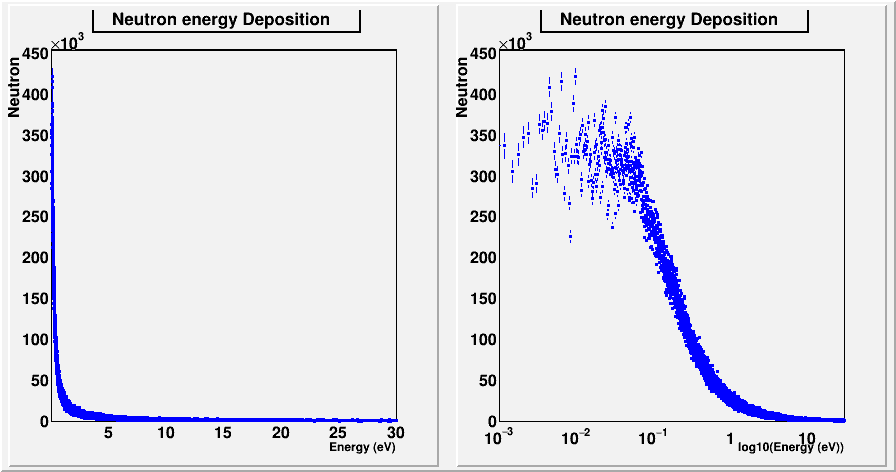
\includegraphics[height=30mm, width=55mm]{../PICS/NeutEdepBIC.png}\label{fig:neutEdepBIC} 
                
                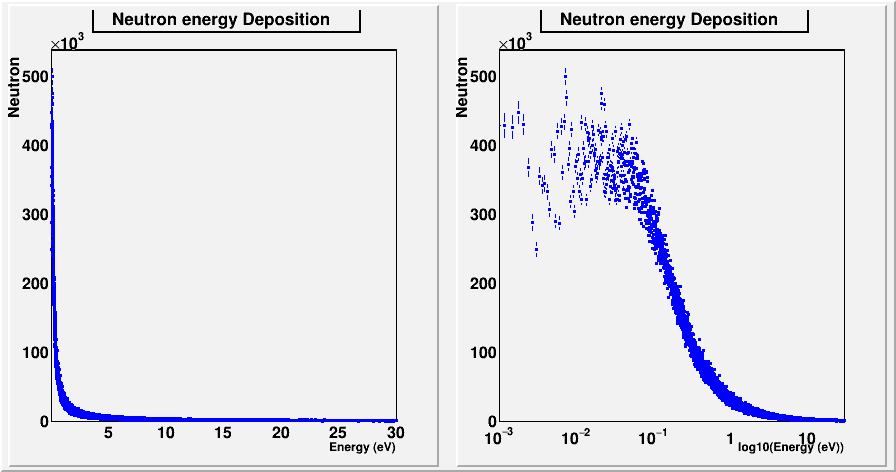
\includegraphics[height=30mm, width=55mm]{../PICS/NeutEdepBERT.png}
                \label{fig:neutEdepBERT} 
            \end{tabular}    
            \caption{Neutron Energy deposition for $QGSP\_BIC\_HP$ and $QGSP\_BERT\_HP$  Physics model.}
        \end{figure}
    \end{frame}

    \begin{frame}
        \frametitle{Distribution of Neutron Energy and Times}
        \begin{figure}
            \begin{tabular}{ll}
                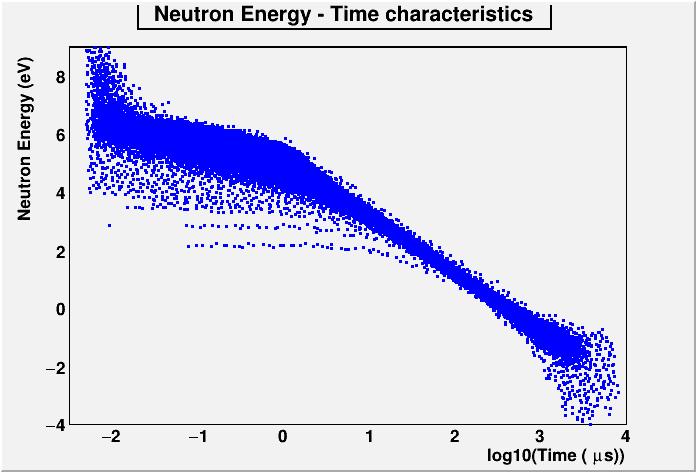
\includegraphics[height=40mm, width=50mm]{../PICS/NeutEnergyTimeBIC.png} \label{fig:NeutETBIC}                
                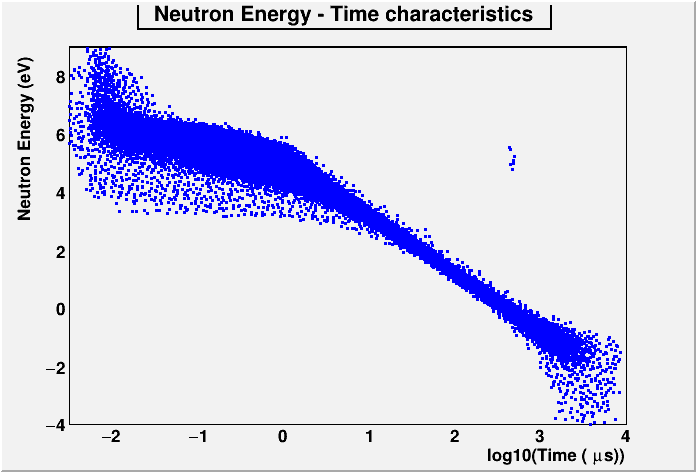
\includegraphics[height=40mm, width=60mm]{../PICS/NeutEnergyTimeBERT.png}
                \label{fig:NeutETBERT}
            \end{tabular}
            \caption{Distribution of Neutron energies and times using $QGSP\_BIC\_HP$  and $QGSP\_BERT\_HP$ physics model.}
        \end{figure}
    \end{frame}

    \begin{frame}
        \frametitle{Distribution of Neutron Energy and Times}
        \begin{figure}
            \begin{tabular}{ll}
                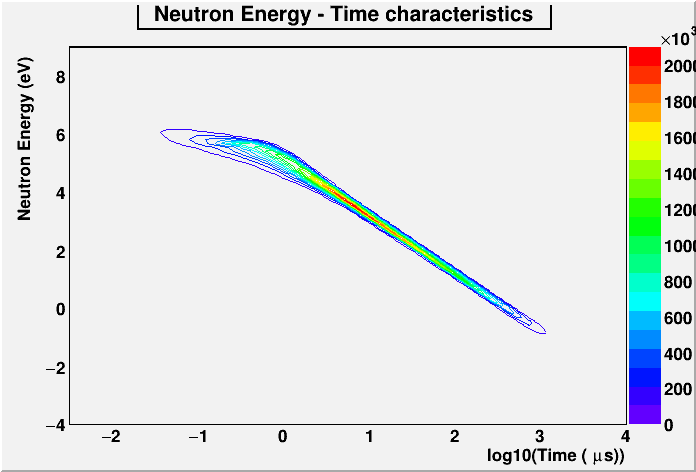
\includegraphics[height=35mm, width=50mm]{../PICS/NeutEnergyTimeCONTBIC.png} \label{fig:NeutETCONTBIC}                
                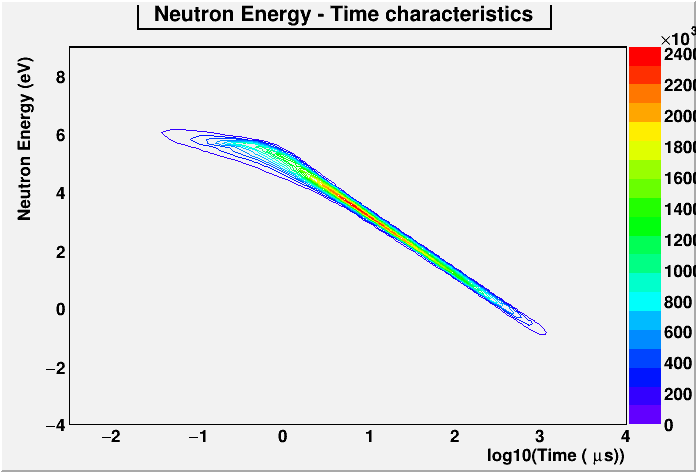
\includegraphics[height=35mm, width=60mm]{../PICS/NeutEnergyTimeCONTBERT.png}
                \label{fig:NeutETCONTBERT}
            \end{tabular}
            \caption{Distribution of Neutron energies and times using $QGSP\_BIC\_HP$ and  $QGSP\_BERT\_HP$ physics model.}
        \end{figure}
    \end{frame}

    \begin{frame}
        \frametitle{Correlation of Neutron Energy and Times}
        \begin{figure}
            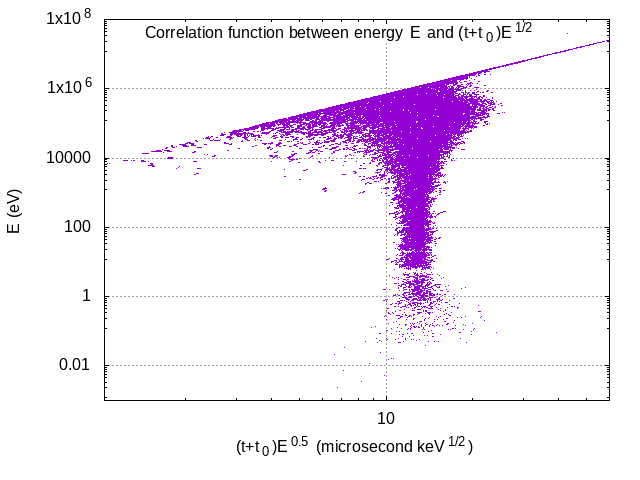
\includegraphics[height=65mm, width=100mm]{../PICS/NeutEnergyTimeCorrBERT.png} \label{fig:NeutETCorrBERT}
            \vskip -5mm                        
            \caption{Correlation between neutron energy $E (eV)$ and $(t+t_0)\sqrt{E}$ using  $QGSP\_BERT\_HP$ physics model. Here $t_0$ $\approx$ 0.37 $\mu s$.}
        \end{figure}
    \end{frame}

    \begin{frame}
        \frametitle{Distribution of Other Particles Energy and Times}
        \begin{figure}
            \begin{tabular}{ll}
                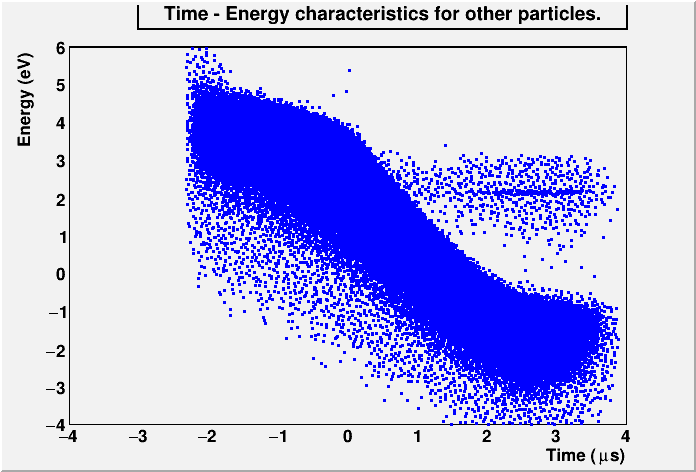
\includegraphics[height=40mm, width=55mm]{../PICS/OtherEnergyTimeBIC.png}
                \label{fig:othETBIC}
                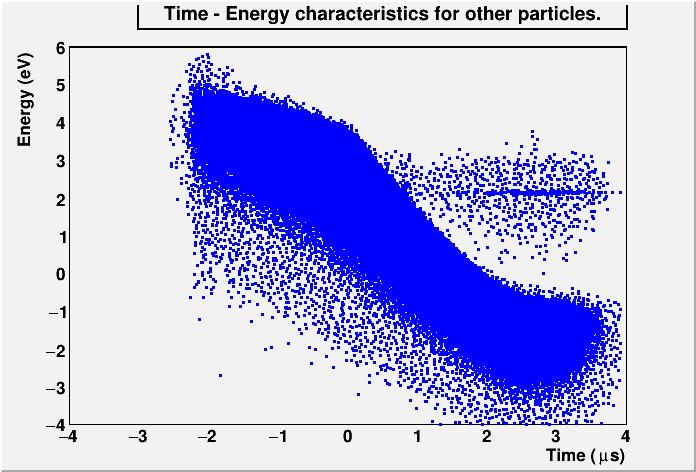
\includegraphics[height=40mm, width=55mm]{../PICS/OtherEnergyTimeBERT.png}
                \label{fig:othETBERT}
            \end{tabular}
            \caption{Distribution of other particles energies and times using $QGSP\_BIC\_HP$ and $QGSP\_BERT\_HP$ physics model.}
        \end{figure}
    \end{frame}

    \begin{frame}
        \frametitle{Distribution of Other Particles Energy and Times}
        \begin{figure}
            \begin{tabular}{ll}
                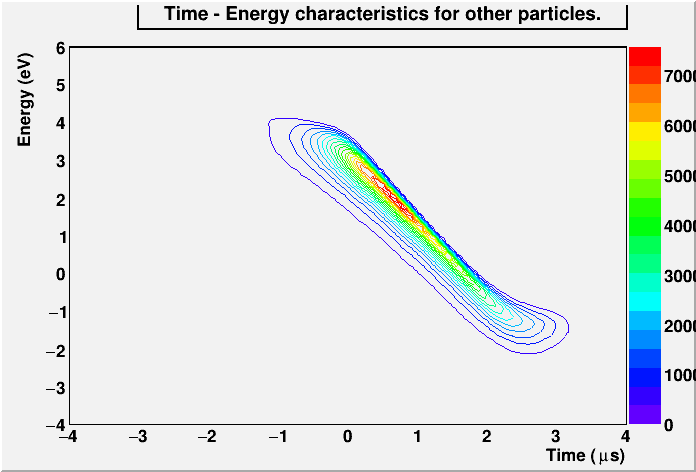
\includegraphics[height=40mm, width=55mm]{../PICS/OtherEnergyTimeCONTBIC.png}
                \label{fig:othETCONTBIC}
                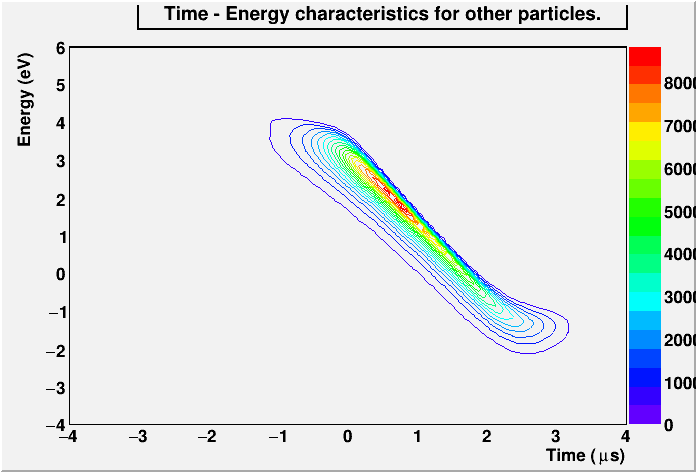
\includegraphics[height=40mm, width=55mm]{../PICS/OtherEnergyTimeCONTBERT.png}
                \label{fig:othETContBERT}
            \end{tabular}
            \caption{Distribution of other particles energies and times using $QGSP\_BIC\_HP$ and $QGSP\_BERT\_HP$ physics model.}
        \end{figure}
    \end{frame}

    \begin{frame}
        \frametitle{Distribution of fluence against energy}
        \begin{figure}
            \begin{tabular}{ll}
                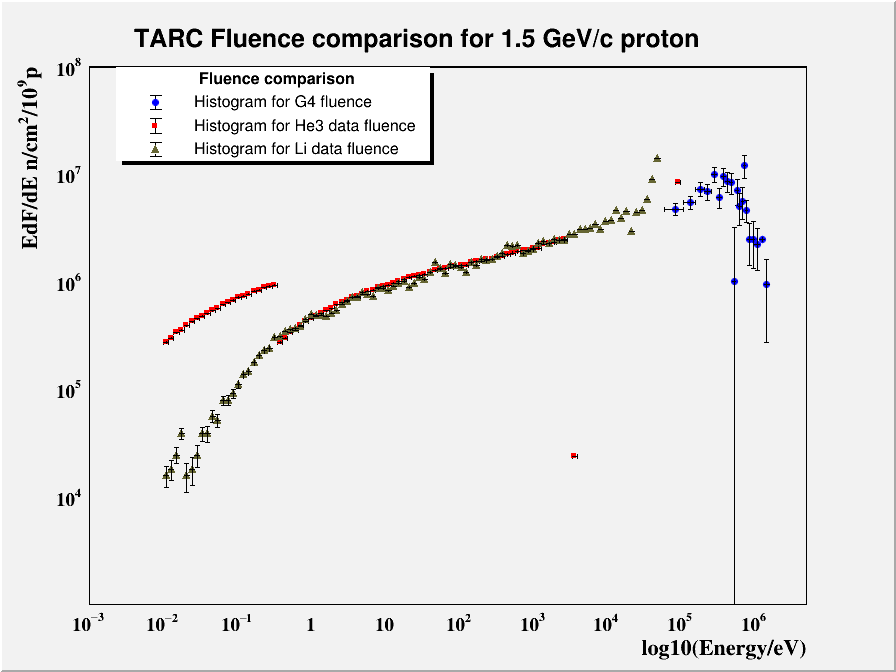
\includegraphics[height=40mm, width=55mm]{../PICS/fluenceBIC.png}\label{fig:flBIC}
                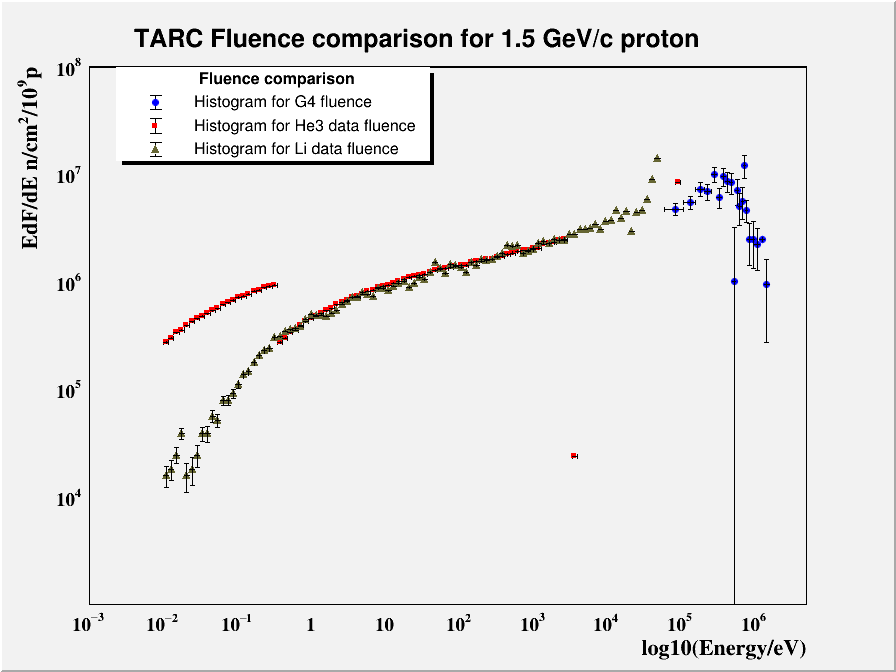
\includegraphics[height=40mm, width=55mm]{../PICS/fluenceBERT.png}\label{fig:flBERT}
            \end{tabular}    
        \caption{Distribution of fluence against energy for $QGSP\_BIC\_HP$ and $QGSP\_BERT\_HP$ physics models.}
        \end{figure}
    \end{frame}

    \begin{frame}
        \frametitle{Distribution of fluence at different radial distance away from the centre.}
        \begin{figure}
            \begin{tabular}{ll}
                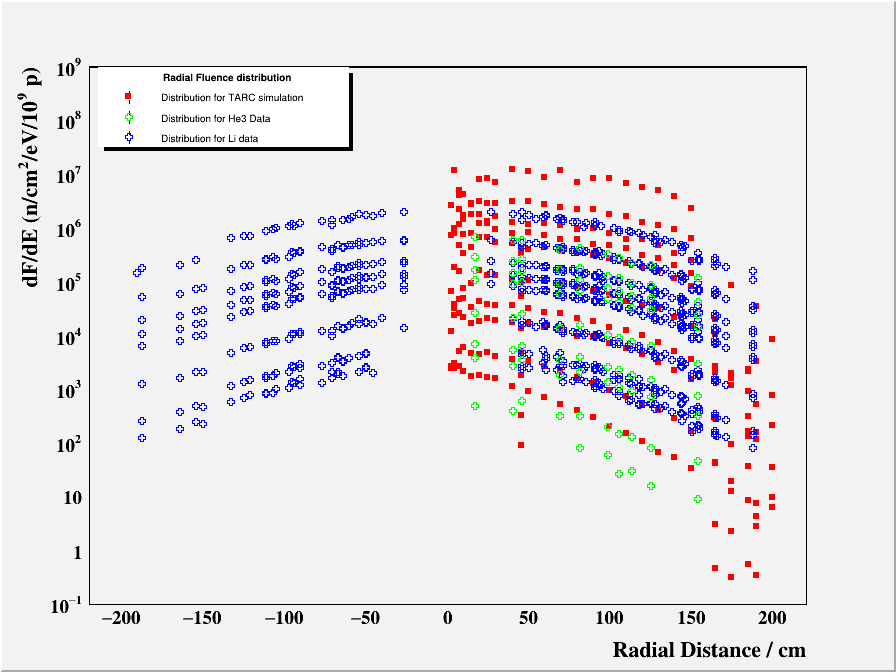
\includegraphics[height=40mm, width=55mm]{../PICS/fluenceRadialBIC.png}\label{flRADBIC}
                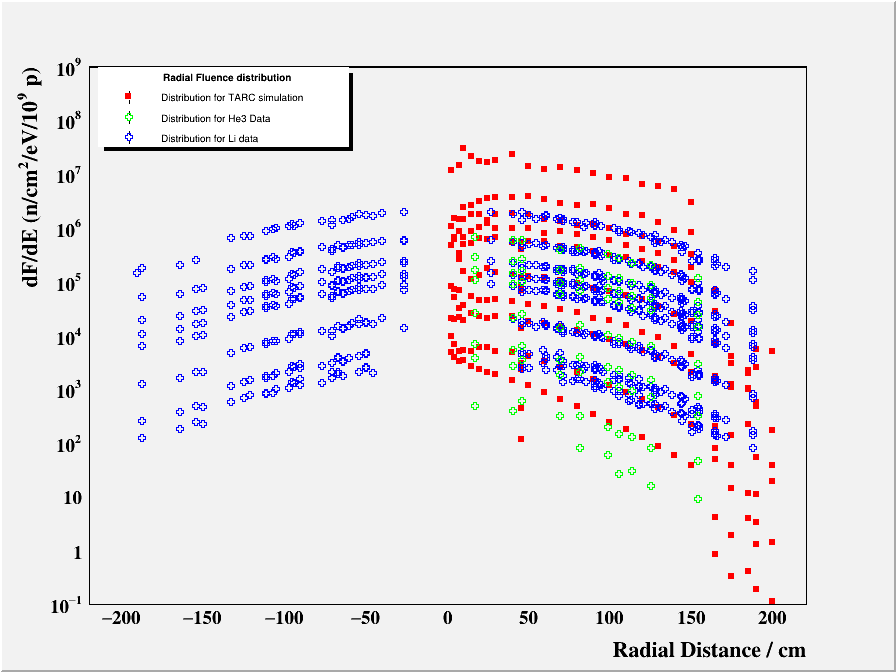
\includegraphics[height=40mm, width=55mm]{../PICS/fluenceRadialBERT.png}\label{flRADBERT}
            \end{tabular}
        \caption{Distribution of fluence against radial distance from the centre using $QGSP\_BIC\_HP$ and $QGSP\_BERT\_HP$ physics models.}
        \end{figure}
    \end{frame}

    \begin{frame}
        \frametitle{Distribution of Ratio of fluence from Geant4 simulation and TARC experimental data}
        \begin{figure}
            \begin{tabular}{cc}
                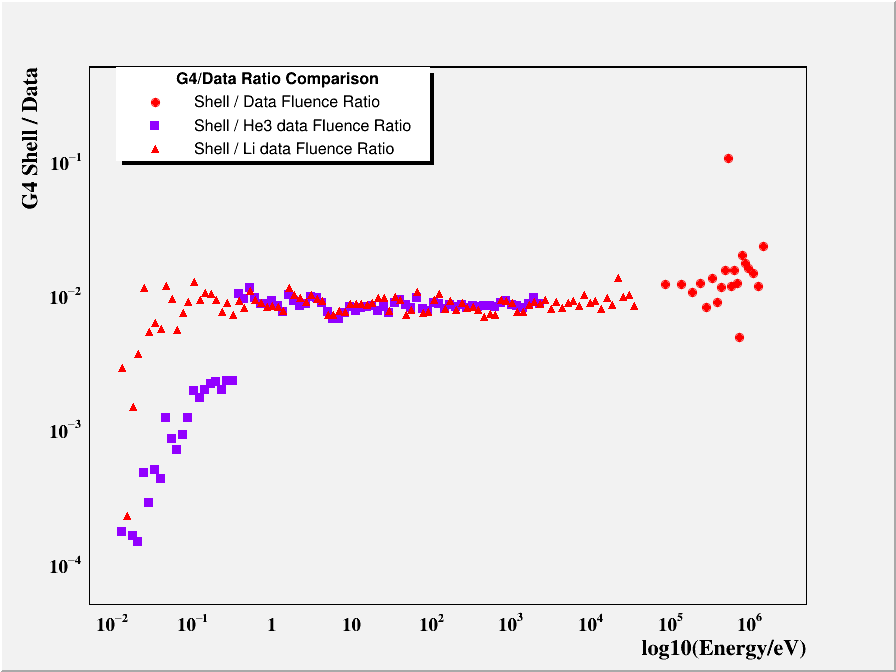
\includegraphics[height=40mm,width=55mm]{../PICS/fluenceRatioBIC.png}\label{fig:flRatBIC}
                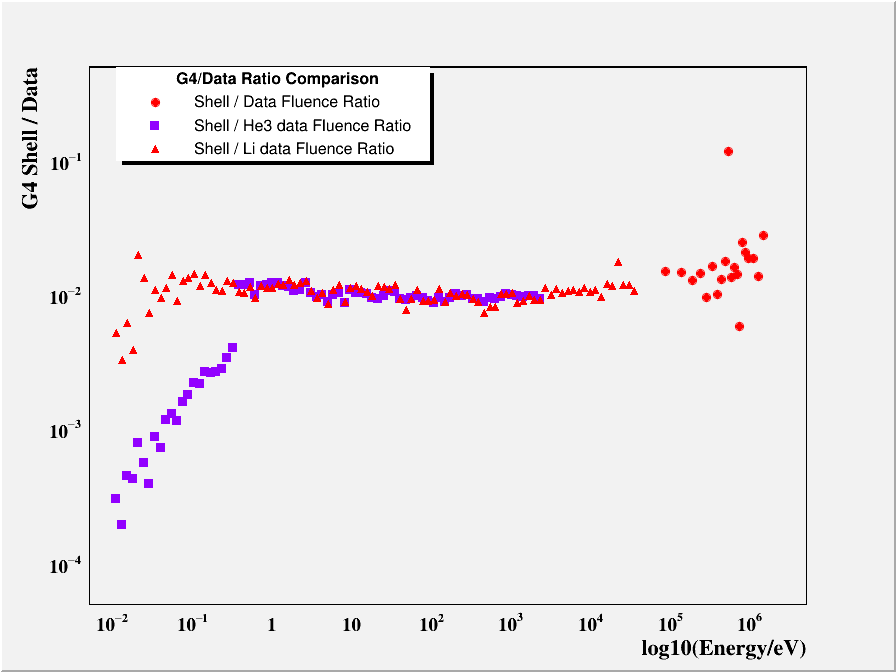
\includegraphics[height=40mm,width=55mm]{../PICS/fluenceRatioBERT.png}\label{fig:flRatBERT}
            \end{tabular}
        \caption{Distribution of ratio of fluence obtained from Geant4 simulation to experimental data using $QGSP\_BIC\_HP$ and $QGSP\_BERT\_HP$ physics models.}
        \end{figure}
    \end{frame}
\end{document}
